\documentclass[sigconf,review]{acmart}

\usepackage{tikz}
\usetikzlibrary{positioning,arrows.meta,fit,backgrounds,calc}
\definecolor{cData}{RGB}{219,234,254}\definecolor{cDataB}{RGB}{37,99,235}
\definecolor{cFeat}{RGB}{220,252,231}\definecolor{cFeatB}{RGB}{22,163,74}
\definecolor{cModel}{RGB}{255,237,213}\definecolor{cModelB}{RGB}{234,88,12}
\definecolor{cEval}{RGB}{237,233,254}\definecolor{cEvalB}{RGB}{124,58,237}

\setlength{\textfloatsep}{7pt plus 2pt minus 2pt}
\setlength{\floatsep}{5pt plus 2pt minus 2pt}
\setlength{\intextsep}{6pt plus 2pt minus 2pt}
\setlength{\abovecaptionskip}{4pt}
\setlength{\belowcaptionskip}{2pt}
\setlength{\abovedisplayskip}{5pt plus 2pt minus 2pt}
\setlength{\belowdisplayskip}{5pt plus 2pt minus 2pt}
\setlength{\abovedisplayshortskip}{3pt plus 2pt minus 2pt}
\setlength{\belowdisplayshortskip}{3pt plus 2pt minus 2pt}

\AtBeginDocument{%
  \providecommand\BibTeX{{Bib\TeX}}}

\setcopyright{none}
\copyrightyear{2026}
\acmYear{2026}
\acmDOI{}
\acmConference[ICAIF '26]{ACM International Conference on AI in Finance}{November 14--17, 2026}{Milan, Italy}
\acmISBN{}

%% ============================================================================
%% v3 -- full reposition for ICAIF '26 (deadline 2026-08-02 AoE).
%% Every number in this file is backed by a committed artifact
%% (TP2MVTransformer/tables/action_list/*, tables/*.json) or by the v2_1 text
%% it revises. Slots that await the collaborator rerun of
%% 67_mlp5_selectivity_and_dsr_fix.py are marked "TODO-RERUN[67]".
%% ============================================================================

\begin{document}

\title{Selection, Not Architecture: An Operating-Point Confound in Evaluating Machine-Learning Trading Strategies}
\subtitle{Evidence from TP2 Violations in SPY American Call Options}

\author{Pawel Polak}
\affiliation{%
  \institution{Stony Brook University}
  \city{Stony Brook}
  \state{New York}
  \country{USA}}
\email{pawel.polak@stonybrook.edu}

\author{Jyotir Manishkumar Patel}
\affiliation{%
  \institution{Stony Brook University}
  \city{Stony Brook}
  \state{New York}
  \country{USA}}
\email{jyotirmanishku.patel@stonybrook.edu}

\author{Omkar Lashkare}
\affiliation{%
  \institution{Stony Brook University}
  \city{Stony Brook}
  \state{New York}
  \country{USA}}
\email{omkarvilas.lashkare@stonybrook.edu}

\renewcommand{\shortauthors}{Polak, Patel, Lashkare}

\begin{abstract}
Shape restrictions on the option surface---here total positivity of order two (TP2)---flag candidate relative-value opportunities, but detecting a violation is not the same as trading one profitably. On SPY American calls, trading every TP2 episode over 2021--2026 loses \$12.52M under a fixed-notional convention (Sharpe $-1.01$): the problem is conditional selection, not detection. Three learned selectors---LightGBM, an MLP, and a transformer attending to prior episodes over five domain-relevant distances---each turn this into a positive out-of-sample return under one causal, untuned rule: trade when the calibrated probability is at least $0.5$.

We use this setting to document an evaluation pathology we argue is general to trading pipelines. Because trades are selected by thresholding a \emph{recalibrated} probability, any change to the model---ensembling, random seed, architecture---silently changes how many trades are taken, so reported risk-adjusted performance conflates model quality with operating point. Five-seed ensembling moves trade count $+75\%$ for the MLP and $-13\%$ for the transformer, and the Sharpe ranking between them reverses. We give the controls that separate the two effects: matched-selectivity curves, seed-dispersion intervals, and a deflated Sharpe ratio over the full 21-configuration search, which no evaluated configuration clears comfortably.

Under these controls the architectural claim does not survive: an $L_2$-regularized logistic regression on the same 48 features matches the 37{,}086-parameter transformer, permuting the attended history costs only 0.04 Sharpe, and the transformer's edge vanishes under capital-constrained sizing. The feature construction, not the architecture, carries the signal.
\end{abstract}

\begin{CCSXML}
<ccs2012>
 <concept>
  <concept_id>10010147.10010257.10010258.10010259</concept_id>
  <concept_desc>Computing methodologies~Machine learning</concept_desc>
  <concept_significance>500</concept_significance>
 </concept>
 <concept>
  <concept_id>10010405.10010481.10010485</concept_id>
  <concept_desc>Applied computing~Economics</concept_desc>
  <concept_significance>300</concept_significance>
 </concept>
</ccs2012>
\end{CCSXML}

\ccsdesc[500]{Computing methodologies~Machine learning}
\ccsdesc[300]{Applied computing~Economics}

\keywords{backtest validation, model selection, ensembling, options, total positivity, statistical arbitrage}

\maketitle

\section{Introduction}
\label{sec:intro}

When two machine-learning trading models are compared on a backtest, the reported ranking is usually read as a statement about the models. This paper documents, in a fully worked empirical setting, a mechanism by which it can instead be a statement about the \emph{evaluation pipeline}. In a standard pipeline---score, recalibrate, threshold, trade---the set of trades taken is an endogenous function of the model: any change to the model (a different architecture, an ensemble of seeds, even a different random initialization) shifts the calibrated score distribution, and with it the number and composition of trades crossing a fixed threshold. Risk-adjusted performance is then evaluated at \emph{different operating points} for different models, and the comparison conflates model quality with selectivity. We call this the \emph{operating-point confound}. It is distinct from, and compounds, the well-documented variance of ML benchmarks across seeds and tuning budgets~\cite{bouthillier2021accounting,dodge2019show,melis2018state,lucic2018gans,agarwal2021deep} and the classical data-snooping problem in backtests~\cite{white2000reality,hansen2005spa,harvey2016crosssection,bailey2014deflated}: it operates even at matched tuning budgets, through the decision rule itself.

Our empirical setting is a relative-value signal on SPY American call options. Total positivity of order two (TP2) is a no-arbitrage-adjacent shape restriction on call prices across strike and maturity~\cite{glasserman2026tp2theory,glasserman2023convexity}; violations flag candidate opportunities~\cite{glasserman2025tp2}. Detection alone is not a strategy: trading every detected T1/K2 episode over the 2021--2026 test years loses \$12.52M under a \$1{,}000-per-trade convention (Sharpe $-1.01$, 2 of 6 years positive). The economic problem is \emph{conditional selection}---deciding which episodes are worth trading---and it is solvable: a LightGBM classifier, an MLP, a historical-attention transformer, and even an $L_2$-regularized logistic regression on the same 48 features each convert the unconditional loss into a substantial positive out-of-sample return under one fixed, causal rule (trade when calibrated probability $\ge0.5$), evaluated on rolling walk-forward splits.

This setting surfaces the confound concretely. Averaging five seeds before recalibration moves the MLP's trade count from 14{,}258 to 24{,}977 ($+75\%$) but the transformer's from 16{,}435 to 14{,}338 ($-13\%$), and the Sharpe ranking between the two architectures reverses (Section~\ref{sec:confound}). The same reversal recurs one level down, between plain attention and an ALiBi-style distance-biased attention variant, and again in a no-history ablation whose apparent effect shrinks by four fifths when moved from one seed to five. None of the underlying gaps is statistically separable at six test years (two-sided sign-test power $\approx0.26$ against a model that truly wins 80\% of years).

Our contributions are:
\begin{enumerate}
\item \textbf{Identification of the operating-point confound.} We show that in a threshold-based trading pipeline, ensembling (or any model change) acts on performance through two channels---the scores and the operating point---and that the second channel alone can reverse a Sharpe ranking. Seed-count-mismatched comparisons, common in applied work, are therefore uncontrolled in a way not captured by the existing benchmarking-variance literature (Section~\ref{sec:confound}).
\item \textbf{A validation protocol that separates the channels.} Matched-selectivity curves (sweeping the threshold to compare models at equal trade count), seed-dispersion intervals with interquartile means~\cite{agarwal2021deep}, two-sided paired tests with explicit power accounting, a trade-dependence-aware block bootstrap~\cite{kunsch1989}, and a deflated Sharpe ratio~\cite{bailey2014deflated} over the \emph{complete} 21-configuration search history, which we disclose (Sections~\ref{sec:selectivity}--\ref{sec:dsr}).
\item \textbf{A documented TP2 episode pipeline for SPY American calls} with cost-aware labels, a per-year characterization of a $\sim$4$\times$ label-base-rate shift, and an explicit accounting of a feature-selection leakage channel that per-fold splitting does not remove (Sections~\ref{sec:data}--\ref{sec:method})---the empirical setting for (1) and (2), in which conditional selection recovers a positive return from an unconditionally unprofitable signal across four independent model families.
\item \textbf{A disciplined negative result on architecture.} Under the controls in (2), the transformer's apparent edge does not survive: a linear model on the same features matches it, attending to \emph{randomly chosen} past episodes performs within 0.04 Sharpe of attending to the most recent ones, and capital-constrained sizing erases its advantage entirely---consistent with the tabular-learning literature~\cite{grinsztajn2022why,shwartzziv2022tabular,gorishniy2021revisiting}. The signal lives in the feature construction, not the architecture (Sections~\ref{sec:ablations},~\ref{sec:capitalscaled}).
\end{enumerate}

\section{Background and Related Work}
\label{sec:related}

\subsection{Benchmark Variance and Data Snooping}
That ML model comparisons are sensitive to seeds, tuning budgets, and reporting choices is established across language modeling~\cite{melis2018state}, GANs~\cite{lucic2018gans}, deep RL~\cite{agarwal2021deep}, and general benchmarking~\cite{bouthillier2021accounting,dodge2019show}. In finance, the multiple-testing problem of backtest research has its own literature: reality checks~\cite{white2000reality}, superior-predictive-ability tests~\cite{hansen2005spa}, the cross-sectional haircut of~\cite{harvey2016crosssection}, and the deflated Sharpe ratio~\cite{bailey2014deflated}. The confound we document is complementary to both lines: it arises \emph{after} scoring, in the decision rule, and persists even when seeds and trials are honestly matched and counted---because the rule silently re-selects the portfolio whenever the score distribution moves.

\subsection{TP2 Inequalities and Options Arbitrage}
TP2 requires the ratio of a higher-strike to a lower-strike call price at the same maturity to increase with time-to-expiry, a property of Black--Scholes and a broad class of arbitrage-free models~\cite{glasserman2026tp2theory,glasserman2023convexity}. A TP2 violation is stronger than the absence of calendar-spread arbitrage and can indicate a relative-value opportunity. Our episode detection and normalized-exposure convention follow the companion SPX study~\cite{glasserman2025tp2}, which finds violations rare, fast-reverting, and tradable. The theorem is proved for European-style cash-settled index options; its conditions do not literally cover American-style SPY on dividend-paying shares~\cite{cosma2020earlyexercise}. We treat TP2 as an empirically testable hypothesis about SPY prices, not an established property (Section~\ref{sec:limitations}).

\subsection{Machine Learning for Options and Tabular Data}
ML for options spans surface fitting, hedging, pricing, and execution-aware trading~\cite{kearns2013mlmicrostructure}, and cross-sectional option-return prediction at scale~\cite{bali2023option}. We pose a narrower problem: binary trade/no-trade classification conditional on a detected violation, scored purely by realized, cost-aware trading performance. Our finding that gradient boosting and a linear model match deep architectures on 48 engineered features is consistent with systematic evidence on tabular data~\cite{grinsztajn2022why,shwartzziv2022tabular,gorishniy2021revisiting}.

\subsection{Attention with Relative Biases}
Relative-position biases are standard alternatives to absolute positional encodings~\cite{shaw2018self,raffel2020t5}, including structural biases over graphs~\cite{ying2021graphormer} and functional schemes for long context~\cite{li2024fire}. ALiBi~\cite{press2022alibi} penalizes attention logits linearly in scalar token distance with fixed per-head slopes. TP2 episodes have no single natural distance, so we test a multivariate generalization (five domain distances, slopes learned per head); its effect on trading performance turns out to be another instance of the operating-point confound (Section~\ref{sec:transformer}).

\section{Data and Episode Construction}
\label{sec:data}

\subsection{Source, Scope, and a Regime Shift}
\label{sec:data-source}
We use SPY American call options 2014--2026 (2013 is excluded as a vendor anomaly: 49{,}090 reported episodes versus 438 in 2014). After the filters below, the modeling universe is 177{,}487 unique episodes spanning 2014-02-03 to 2026-06-04. Table~\ref{tab:peryear} reports per-year episode counts, candidate episode-strategy pairs (two per episode), and the profitable-label base rate $\pi_t$. Two facts matter downstream. First, episode frequency is highly non-stationary, rising by two orders of magnitude across the sample. Second, $\pi_t$ collapses from 45--73\% in 2017--2020 to 11--16\% in 2021--2026: pair-weighted, the first four folds train at base rates of 39.9\%, 61.3\%, 46.8\%, and 43.4\% but test at 14.5--16.0\%, while the last two folds are nearly matched (15.4\%/15.6\% training versus 11.1\% test). The only pipeline component that adapts to this shift is a one-year isotonic calibration (Section~\ref{sec:calibration}); consistent with the shift being concentrated in the early folds, the identical fixed rule earns Sharpe 1.17 on the 2021--2023 half and 2.88 on the 2024--2026 half.

\begin{table}[t]
\centering
\footnotesize
\begin{tabular}{rrrr@{\hskip 1.4em}rrrr}
\toprule
Yr & Epis. & Pairs & $\pi_t$ & Yr & Epis. & Pairs & $\pi_t$ \\
\midrule
2014 & 438 & 876 & 8.6\% & 2021 & 20{,}588 & 41{,}176 & 15.8\% \\
2015 & 140 & 280 & 1.1\% & 2022 & 6{,}604 & 13{,}208 & 16.0\% \\
2016 & 3{,}786 & 7{,}572 & 5.4\% & 2023 & 12{,}731 & 25{,}462 & 14.5\% \\
2017 & 12{,}284 & 24{,}568 & 45.8\% & 2024 & 34{,}167 & 68{,}334 & 15.9\% \\
2018 & 5{,}969 & 11{,}938 & 26.6\% & 2025 & 41{,}577 & 83{,}154 & 11.1\% \\
2019 & 4{,}151 & 8{,}302 & 41.6\% & 2026$^\dagger$ & 9{,}335 & 18{,}670 & 11.1\% \\
2020 & 25{,}717 & 51{,}434 & 72.5\% & & & & \\
\bottomrule
\end{tabular}
\caption{T1/K2 episodes, candidate pairs, and profitable-label base rate $\pi_t$ by year. $\pi_t$ collapses $\sim$4$\times$ between the 2017--2020 training regime and the 2021--2026 test regime. $^\dagger$2026 ends 2026-06-04 ($\approx$107 trading days); Section~\ref{sec:robustness} re-runs all metrics without it.}
\label{tab:peryear}
\end{table}

\subsection{Episode Detection and Tracking}
\label{sec:episode-tracking}
A TP2 episode begins when a conservative bid/ask price rectangle violates $C(K_1,T_1)\,C(K_2,T_2) < C(K_1^{\ast},T_2)\,C(K_2^{\ast},T_1)$ for strikes $K_1<K_2$ and maturities $T_1<T_2$, with rounded-up adjusted strikes $K^{\ast}$ where no exact match exists. Unlike~\cite{glasserman2025tp2} we do not additionally filter against a vertical/calendar-spread no-arbitrage condition (reported there to remove under 2\% of violations with minimal effect); we list this as a limitation rather than assume it away. The raw detector output is daily and rectangle-level; treating each daily row as independent would inflate the sample, so consecutive appearances of the same strike/maturity pair are grouped into one episode keyed on the near-leg strike and maturity. Over the full history, 2{,}430{,}220 daily rows collapse to 2{,}098{,}213 pair episodes; 88.66\% are single-session, median duration is one session, the maximum is 14, and 50.6\% end in true reversion. The 177{,}487-episode modeling universe is the downstream conservative bid/ask, T1/K2, cost-labeled subset.

We also build a lifecycle panel following every episode over a fixed event-time window (20 pre-event sessions through expiration; Figure~\ref{fig:lifecyclepath}): normalized TP2 pressure is flat pre-event, spikes at day 0 by construction, and decays toward zero. Although the panel runs through expiration, every lifecycle feature used as model input is truncated at event day 0---only pre- and at-signal pressure, observability, and liquidity summaries enter the feature set, never post-signal rows.

\begin{figure}[t]
\centering
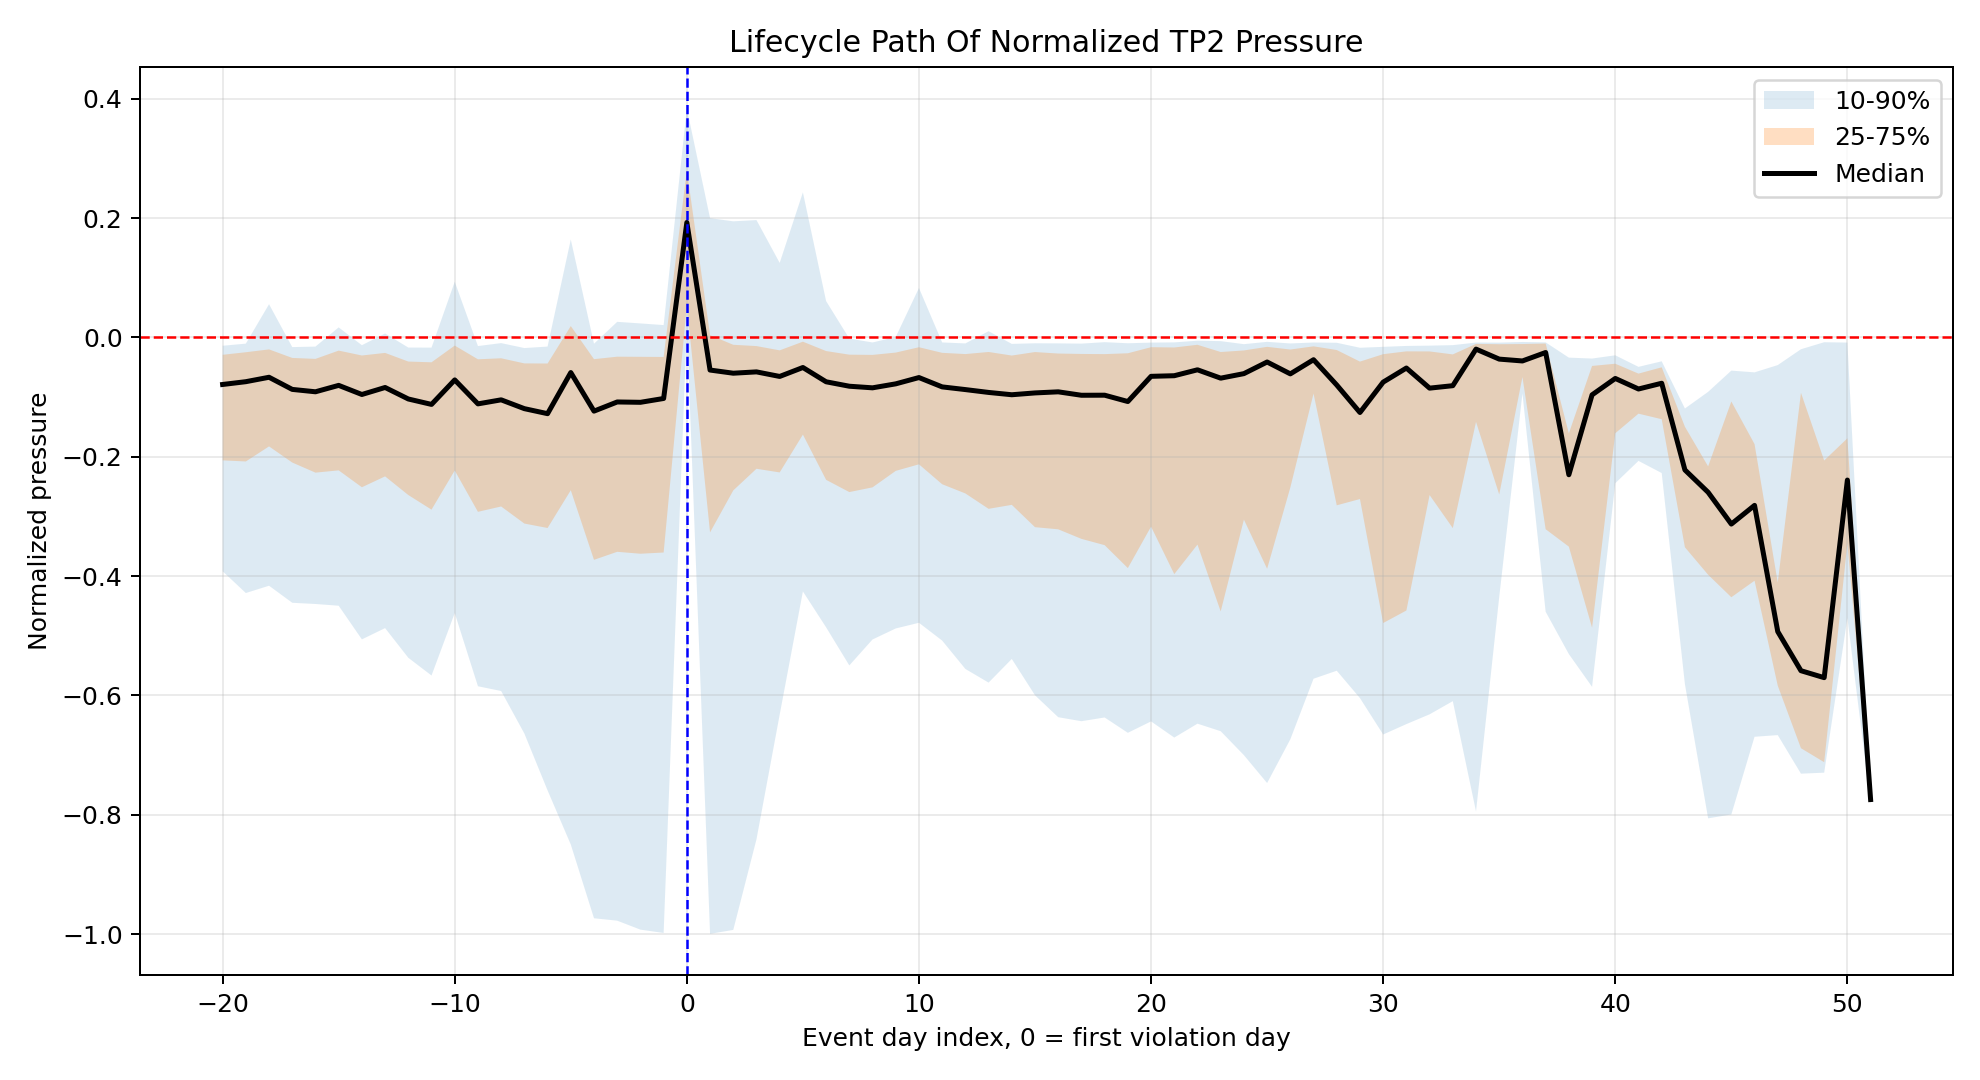
\includegraphics[width=0.62\linewidth]{figures/lifecycle_normalized_pressure_band.png}
\caption{Normalized TP2 pressure---$(C(K_1^{\ast},T_2)C(K_2^{\ast},T_1)-C(K_1,T_1)C(K_2,T_2))$ over the sum of both sides---from 20 sessions before first violation through expiration, all conservative episodes 2014--2026. Solid: median; bands: 10--90 and 25--75 percentiles; dashed: event day 0.}
\label{fig:lifecyclepath}
\end{figure}

\subsection{Labels, Costs, and the T1/K2 Restriction}
\label{sec:labels}
The label policy holds positions to expiration and books the terminal intrinsic payoff of the selected leg. Hold-to-expiry is the structurally natural primary policy because 88.66\% of episodes are single-session: most never present a distinct post-signal reversion exit, and the 171 selected trades that do carry a defined true-reversion exit are too few to adjudicate an alternative exit policy empirically.
%% TODO-RERUN[67]: if the paired reversion-vs-expiry comparison on those 171 is
%% computed and committed, replace the clause above with its result.
Realized returns are cost-aware: the entry leg executes at the full bid/ask spread (buy at ask, sell at bid) plus a \$0.65-per-contract commission per leg, matching Interactive Brokers' published IBKR Lite schedule.\footnote{\url{https://www.interactivebrokers.com/en/pricing/commissions-options.php}, accessed 2026.} Returns are normalized by each trade's own gross exposure and expressed via a \$1{,}000 fixed-exposure convention (raw exposures range from a median of \$7--\$11 to \$814{,}000). We restrict to the T1 and K2 denominations, both shorting the shorter-dated leg---a structural prior fixed before training, since T2/K1 short the longer-dated leg and face a longer horizon for adverse moves. The prior is confirmed empirically: an unrestricted four-denomination LightGBM loses \$37.23M (Sharpe $-1.76$, 1/6 positive years).

\section{Models and Evaluation Protocol}
\label{sec:method}

Figure~\ref{fig:pipeline} summarizes the full pipeline from raw quotes to evaluated portfolio; the subsections below specify each stage.

\begin{figure*}[t]
\centering
\resizebox{0.82\textwidth}{!}{%
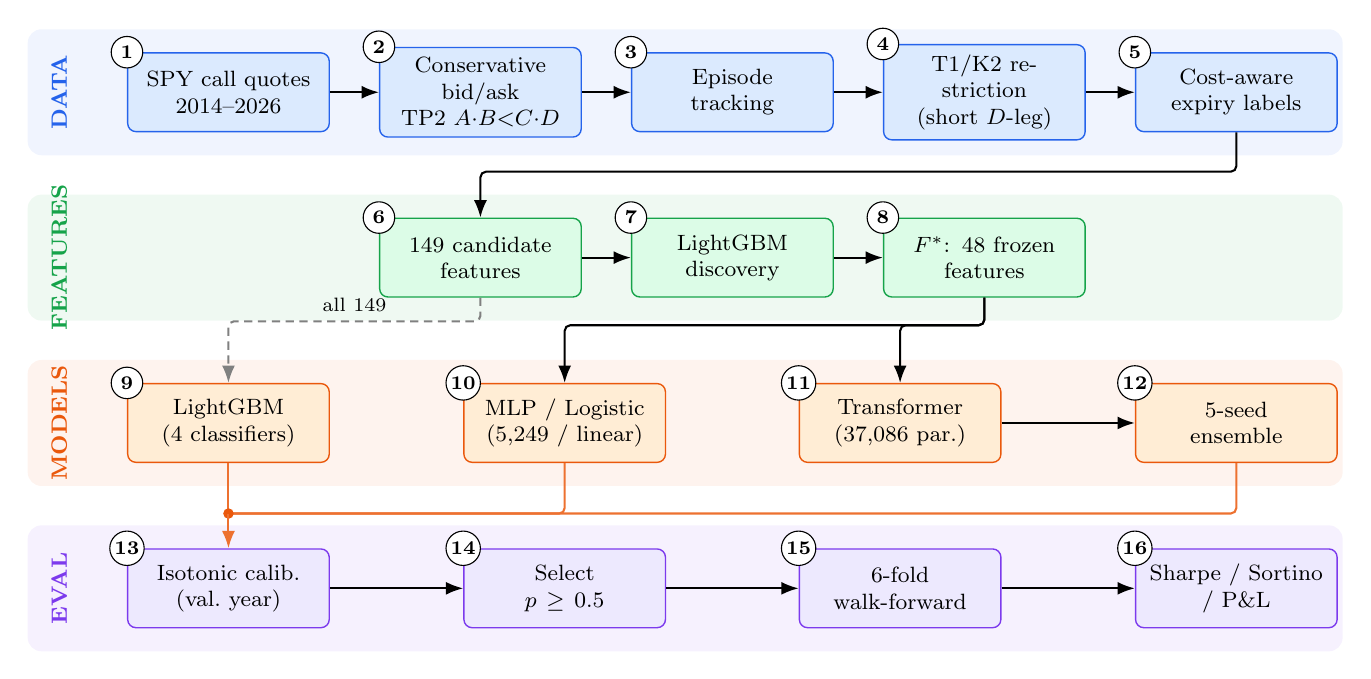
\begin{tikzpicture}[
  every node/.style={font=\footnotesize},
  b/.style={draw, rounded corners=3pt, align=center, text width=2.3cm, minimum height=1.0cm, inner sep=1.3mm, line width=0.5pt},
  bd/.style={b, fill=cData, draw=cDataB}, bf/.style={b, fill=cFeat, draw=cFeatB},
  bm/.style={b, fill=cModel, draw=cModelB}, be/.style={b, fill=cEval, draw=cEvalB},
  arr/.style={-{Latex[length=2.2mm]}, line width=0.75pt, rounded corners=2pt},
  mrg/.style={line width=0.75pt, rounded corners=2pt, cModelB!85},
  brc/.style={-{Latex[length=2.2mm]}, line width=0.75pt, densely dashed, gray, rounded corners=2pt},
  sn/.style={circle, draw, fill=white, font=\scriptsize\bfseries, inner sep=0.3mm, minimum size=4mm}
]
\def\ry{0}\def\rf{-2.1}\def\rm{-4.2}\def\re{-6.3}
\begin{scope}[on background layer]
  \fill[cDataB!7,  rounded corners=5pt] (-2.55,0.80)  rectangle (14.15,-0.80);
  \fill[cFeatB!7,  rounded corners=5pt] (-2.55,-1.30) rectangle (14.15,-2.90);
  \fill[cModelB!7, rounded corners=5pt] (-2.55,-3.40) rectangle (14.15,-5.00);
  \fill[cEvalB!7,  rounded corners=5pt] (-2.55,-5.50) rectangle (14.15,-7.10);
\end{scope}
\node[bd] (n1) at (0,\ry)    {SPY call quotes\\2014--2026};
\node[bd] (n2) at (3.2,\ry)  {Conservative bid/ask\\TP2 $A{\cdot}B{<}C{\cdot}D$};
\node[bd] (n3) at (6.4,\ry)  {Episode\\tracking};
\node[bd] (n4) at (9.6,\ry)  {T1/K2 restriction\\(short $D$-leg)};
\node[bd] (n5) at (12.8,\ry) {Cost-aware\\expiry labels};
\node[bf] (n6) at (3.2,\rf) {149 candidate\\features};
\node[bf] (n7) at (6.4,\rf) {LightGBM\\discovery};
\node[bf] (n8) at (9.6,\rf) {$F^{\ast}$: 48 frozen\\features};
\node[bm] (n9)  at (0,\rm)    {LightGBM\\(4 classifiers)};
\node[bm] (n10) at (4.27,\rm) {MLP / Logistic\\(5{,}249 / linear)};
\node[bm] (n11) at (8.53,\rm) {Transformer\\(37{,}086 par.)};
\node[bm] (n12) at (12.8,\rm) {5-seed\\ensemble};
\node[be] (n13) at (0,\re)    {Isotonic calib.\\(val.\ year)};
\node[be] (n14) at (4.27,\re) {Select\\$p\!\ge\!0.5$};
\node[be] (n15) at (8.53,\re) {6-fold\\walk-forward};
\node[be] (n16) at (12.8,\re) {Sharpe / Sortino\\/ P\&L};
\draw[arr] (n1)--(n2); \draw[arr] (n2)--(n3); \draw[arr] (n3)--(n4); \draw[arr] (n4)--(n5);
\draw[arr] (n5.south) -- ++(0,-0.5) -| (n6.north);
\draw[arr] (n6)--(n7); \draw[arr] (n7)--(n8);
\draw[arr] (n8.south) -- ++(0,-0.35) -| (n11.north);
\draw[arr] (n8.south) -- ++(0,-0.35) -| (n10.north);
\draw[brc] (n6.south) -- ++(0,-0.3) -| (n9.north) node[pos=0.25,above,black,font=\scriptsize]{all 149};
\draw[arr] (n11)--(n12);
\coordinate (jn) at (0,-5.35);
\draw[mrg] (n10.south) |- (jn);
\draw[mrg] (n12.south) |- (jn);
\draw[mrg] (n9.south) -- (jn);
\fill[cModelB] (jn) circle (1.9pt);
\draw[arr, cModelB!85] (jn) -- (n13.north);
\draw[arr] (n13)--(n14); \draw[arr] (n14)--(n15); \draw[arr] (n15)--(n16);
\foreach \n/\l in {n1/1,n2/2,n3/3,n4/4,n5/5,n6/6,n7/7,n8/8,n9/9,n10/10,n11/11,n12/12,n13/13,n14/14,n15/15,n16/16}
  \node[sn] at (\n.north west) {\l};
\node[rotate=90, cDataB,  font=\bfseries\footnotesize] at (-2.15,\ry) {DATA};
\node[rotate=90, cFeatB,  font=\bfseries\footnotesize] at (-2.15,\rf) {FEATURES};
\node[rotate=90, cModelB, font=\bfseries\footnotesize] at (-2.15,\rm) {MODELS};
\node[rotate=90, cEvalB,  font=\bfseries\footnotesize] at (-2.15,\re) {EVAL};
\end{tikzpicture}
}
\caption{Pipeline, steps 1--16. Steps 1--5 build the episode dataset; steps 7--8 select the frozen $F^{\ast}$ dictionary (the pooled selection whose leakage Section~\ref{sec:features} discloses); LightGBM (step 9) trains on all 149 candidates (dashed). All scorers converge on one shared downstream---calibration, $p\ge0.5$ selection, walk-forward evaluation---so the operating-point confound of Section~\ref{sec:confound} arises in the shared stage, not in any model-specific code path.}
\label{fig:pipeline}
\end{figure*}

\subsection{Walk-Forward Design}
We use six rolling folds---three training years, one validation year, one test year---covering test years 2021--2026 (Table~\ref{tab:folds}). Within each fold, feature scaling is fit on training years only and calibration on the validation year only; no test-year information enters either. An expanding-window alternative is evaluated in Section~\ref{sec:robustness}.

\begin{table}[t]
\centering
\footnotesize
\begin{tabular}{lll}
\toprule
Train years & Validation year & Test year \\
\midrule
2017--2019 & 2020 & 2021 \\
2018--2020 & 2021 & 2022 \\
2019--2021 & 2022 & 2023 \\
2020--2022 & 2023 & 2024 \\
2021--2023 & 2024 & 2025 \\
2022--2024 & 2025 & 2026 \\
\bottomrule
\end{tabular}
\caption{Rolling walk-forward folds used for every model and result: train, calibrate (isotonic) on the validation year, evaluate once on the test year.}
\label{tab:folds}
\end{table}

\subsection{Feature Selection, and a Leakage We Disclose}
\label{sec:features}
From 149 candidate features in eight semantic blocks (market, short-leg structure, option risk, surface location, liquidity, TP2 geometry, strategy/calendar, lifecycle pressure), we select 48 features $F^{\ast}$ using LightGBM~\cite{ke2017lightgbm} as a discovery tool: a composite of gain importance, permutation importance, and a temporal-stability score (the fraction of fold$\times$strategy runs placing a feature in the top 30). Only feature \emph{values} feed the downstream models; LightGBM's predictions and importances are never inputs, so the comparison in Section~\ref{sec:results} is between independent selectors on a shared, inspectable dictionary, not a stacked ensemble.

$F^{\ast}$ is selected \emph{once}, pooled over all six folds, and frozen. This is a leakage channel that the per-fold split does not remove, and it is wider than a validation-side effect: the pooled folds train on 2021--2024 and validate on 2020--2025, so every test year except 2026 contributes to the selection of the feature set later used to trade it. The per-fold results of Section~\ref{sec:results} are therefore conditionally out-of-sample given $F^{\ast}$, not unconditionally. Closing this channel requires re-selecting features within each fold (or from a 2017--2019-only window, clean with respect to every test year); we flag it as the pipeline's main unresolved validity issue rather than describing the pipeline as leakage-free.
%% TODO-RERUN[67-followup]: if the 2017-2019-only F* control is run and headline
%% results hold, add one sentence here reporting that the leakage is not
%% load-bearing.

\noindent\textbf{Implementation (all models).} Every model uses the six folds, training-set standardization, validation-year isotonic calibration, and $p\ge0.5$ selection; single-seed rows use the fixed default seed 42 (set a priori, not best-of-several---though Section~\ref{sec:confound} shows it happens to be the MLP's most favorable seed, which is part of the point), and 5-seed ensembles average raw probabilities over seeds \{42,101,202,303,404\} before one calibration. LightGBM: 350 trees, learning rate 0.04, 31 leaves, min-child 30, sub/colsample 0.8, balanced class weights. MLP (48-64-32-1, ReLU, 5{,}249 parameters): Adam, lr $10^{-3}$, $L_2$ $10^{-4}$, batch 1024, $\le$80 epochs, patience 8. Transformer (37{,}086 parameters): hidden 64, 4 heads, $\le$64 history tokens, AdamW lr $3{\times}10^{-5}$, weight decay $10^{-4}$, 8\% warm-up, grad-clip 1.0, $\le$25 epochs, validation-\emph{loss} checkpointing (an earlier ranking-metric checkpoint allowed calibration-degrading epochs to survive), plus a Huber auxiliary loss on realized return. An $L_2$-regularized logistic regression on $F^{\ast}$ serves as the linear floor.

\subsection{The Transformer, Its Distance-Biased Variant, and Ablations}
\label{sec:transformer}
Each candidate episode-strategy pair is a token combining its $F^{\ast}$ values, a strategy embedding, and calendar features. The token cross-attends to the 64 most recently dated episode tokens from strictly earlier calendar days---selected by date alone, never by label or outcome, zero-padded when fewer exist---with logits
$a^{h}_{ij}=q_i\!\cdot\!k_j/\sqrt{d}\,+\,\text{(same/cross-strategy bonus)}$.

\noindent\textbf{MV-ALiBi variant.} Generalizing ALiBi's scalar penalty~\cite{press2022alibi}, we subtract $m_h^{\top}d_{ij}$ from the logit, where $d_{ij}$ collects five domain distances between episodes $i,j$ (time, surface location, short-leg structure, liquidity, lifecycle stage) and $m_h$ is a softplus-positive learned slope vector (20 extra parameters). The mechanism trains as designed: despite $\sim$7:1 raw scale differences across distances, learned slopes converge to 0.26--0.27 for every distance, head, and seed (30 models). Its \emph{trading} effect, however, is ensembling-dependent: at single seed plain attention wins (Sharpe 1.73 vs.\ 1.51), at five seeds the ranking reverses (2.18 vs.\ 2.36; rows in Table~\ref{tab:consolidated}), and neither gap is significant (two-sided sign tests $p=0.219$ and $p=1.000$; block-bootstrap CIs $[-\$162\text{K},\$405\text{K}]$ and $[-\$135\text{K},\$110\text{K}]$). We evaluate plain attention as primary for simplicity while noting the five-seed evidence favors the variant---a first instance of the confound of Section~\ref{sec:confound}.

\noindent\textbf{No-history and permuted-history ablations.}
\label{sec:ablations}
Removing cross-attention entirely (input projection straight to the head; 16{,}130 parameters) looks decisive at matched single seed---Sharpe 1.73$\to$0.87, positive years 6/6$\to$4/6---but at matched \emph{five-seed} ensembles the gap shrinks to 2.18 vs.\ 1.81 (\$719.9K, 6/6): a real but modest $\approx$0.37, one fifth of the single-seed impression. More telling, a variant keeping all 37{,}086 parameters but attending to 64 \emph{randomly chosen} strictly-earlier episodes reaches 2.14 at five seeds---within 0.04 of the full model. The attention pathway helps; \emph{which} history it attends to barely matters. We accordingly do not claim the historical-attention design as a source of edge.

\subsection{Calibration and the Trade-Selection Rule}
\label{sec:calibration}
Isotonic regression~\cite{zadrozny2002transforming} is fit on validation-year predictions only and applied unchanged to the test year; ensembles average raw seed probabilities before one calibration fit. The calibrator family is not decisive but not free either: refitting per fold with Platt scaling instead selects a nearly identical set ($N$ within 0.3\%; test ECE 0.072 vs.\ 0.075) yet shifts Sharpe from 1.79 to 1.66 and P\&L by $-5.8\%$---a $\sim$7\% Sharpe sensitivity we report rather than average away.
%% TODO-RERUN[67]: confirm which configuration the platt-vs-isotonic totals
%% (N=20,125) correspond to and name it here.
The selected count itself carries sampling uncertainty: block-bootstrapping trading dates gives 95\% CIs of roughly $\pm25$--30\% on $N$ (five-seed transformer 14{,}338, CI $[10.3\text{K},19.0\text{K}]$; five-seed MLP $[19.3\text{K},31.6\text{K}]$; LightGBM $[14.8\text{K},25.6\text{K}]$).

The rule itself: trade an episode when its calibrated probability is at least $0.5$, else skip---causal by construction, depending only on the current trade's own probability, identical across models and folds. The \emph{threshold value} is the natural boundary for a calibrated probability and was fixed in advance; we do not, however, claim the rule embodies zero researcher degrees of freedom, because eight alternative selection rules (a validation-tuned threshold, a non-causal top-$K$ fraction at three settings, and probability floors at three settings) were evaluated on the same test window during development, rejected, and are counted as trials in the deflated Sharpe ratio of Section~\ref{sec:dsr}. As a diagnostic, the fixed rule is solidly profitable on both the 2021--2023 and 2024--2026 halves (Sharpe 1.17 and 2.88).

\section{Results}
\label{sec:results}

All results use the identical protocol: validation-only isotonic calibration, the $p\ge0.5$ rule, and daily-grouped metrics from one code path. The annualized Sharpe is $\sqrt{252}\,\bar r_d/\sigma(r_d)$ over per-day summed normalized P\&L on days with at least one selected trade; Sortino replaces $\sigma$ with the standard deviation of negative-P\&L days. Because $\sigma(r_d)$ scales with trades per day, this statistic is \emph{not} directly comparable across models with very different trade counts $N$---the quantitative motivation for the matched-selectivity analysis of Section~\ref{sec:selectivity}.

\subsection{Unconditional Baseline and the Consolidated Comparison}
Trading all 250{,}004 valid episode-strategy pairs (two per episode) over 2021--2026 loses \$12.52M (Sharpe $-1.01$, Sortino $-2.12$, max drawdown $-\$24.51$M, win rate 12.9\%, 2/6 positive years). Every learned selector clears this floor by a wide margin (Table~\ref{tab:consolidated}). Two reference rows bracket the result. An $L_2$ logistic regression on $F^{\ast}$ earns \$2.02M (Sharpe 2.27)---above LightGBM and both single-seed deep models---so most of the tradable signal is \emph{linear in the selected features}~\cite{grinsztajn2022why,shwartzziv2022tabular}. Random selection at the MLP's trade count loses \$0.77M (Sharpe $-1.14$), so the gains are not a mechanical consequence of taking fewer trades.

\begin{table}[t]
\centering
\footnotesize
\resizebox{\linewidth}{!}{%
\begin{tabular}{llrrrrrrrr}
\toprule
Method & Seeds & Trades & Total P\&L & Sharpe & Sortino & Win\% & $\bar r$\% & Skew & Pos.\ yrs \\
\midrule
Unconditional & -- & 250{,}004 & $-$\$12.52M & $-$1.01 & $-$2.12 & 12.9 & $-$5.0 & 16.6 & 2/6 \\
LightGBM & 1 & 19{,}636 & \$682K & 1.25 & 1.12 & 50.6 & 3.5 & 9.4 & 5/6 \\
MLP & 1 & 14{,}258 & \$1.41M & 2.60 & 6.89 & 54.0 & 9.9 & 9.6 & 6/6 \\
MLP & 5 & 24{,}977 & \$3.43M & 1.66 & 6.12 & 33.0 & 13.7 & 8.9 & 4/6 \\
Transformer (plain) & 1 & 16{,}435 & \$686K & 1.73 & 1.70 & 57.9 & 4.2 & 1.1 & 6/6 \\
Transformer (plain) & 5 & 14{,}338 & \$695K & 2.18 & 2.98 & 60.0 & 4.8 & 1.8 & 6/6 \\
Transformer (ALiBi) & 1 & 15{,}015 & \$570K & 1.51 & 1.24 & 61.0 & 3.8 & $-$2.3 & 6/6 \\
Transformer (ALiBi) & 5 & 14{,}648 & \$704K & 2.36 & 3.72 & 60.1 & 4.8 & 1.0 & 6/6 \\
\midrule
Logistic (L2) & 1 & 13{,}841 & \$2.02M & 2.27 & 4.20 & 53.5 & 14.6 & 5.5 & 5/6 \\
Random @$N$ & -- & 14{,}258 & $-$\$0.77M & $-$1.14 & -- & -- & -- & -- & -- \\
\bottomrule
\end{tabular}%
}
\caption{All models and seed counts, plus unconditional, linear, and random-at-matched-$N$ baselines, 2021--2026. `Seeds': independently trained models whose raw probabilities are averaged before one calibration. $\bar r$\%: mean per-trade normalized return; dollar figures under the \$1{,}000-per-trade convention. The two most profitable rows (MLP-5, Logistic) also carry the highest right-skew and lowest win rates: P\&L concentrated in outsized winners, which Sharpe penalizes and Sortino rewards.}
\label{tab:consolidated}
\end{table}

\subsection{The Operating-Point Confound}
\label{sec:confound}
Ensembling acts through two channels at once. It changes the scores---and, because a single isotonic map is refit on the averaged validation probabilities and the threshold stays at $0.5$, it changes \emph{how many trades cross}: $+75\%$ for the MLP (14{,}258$\to$24{,}977), $-13\%$ for the transformer (16{,}435$\to$14{,}338). The two architectures are therefore compared at different points of their own selectivity curves before and after ensembling. On flat-notional Sharpe the ranking reverses (MLP 2.60$\to$1.66; transformer 1.73$\to$2.18), yet on total P\&L, mean per-trade return, and the capital-scaled backtest of Section~\ref{sec:capitalscaled} the MLP leads at \emph{both} seed counts: the ``reversal'' exists on exactly one metric under exactly one sizing convention, driven partly by a payoff-shape change Sharpe penalizes (MLP-5's win rate falls to 33\% while $\bar r$ rises to 13.7\%---more right-skew).

Seed dispersion completes the picture. Across the same five seeds, single-seed MLP Sharpe spans 1.47--2.60 (median 2.07, IQM 2.07)---the 2.60 in Table~\ref{tab:consolidated} is the a-priori default seed 42, which happens to be the most favorable, and the spread exceeds the nominal single-versus-ensemble gap. The transformer is tighter (1.50--1.81, IQM 1.73), and its five-seed ensemble (2.18) beats \emph{every} single seed: ensembling helps the transformer consistently, while the MLP's single-seed point estimate is too noisy to rank architectures on at all.

Formal tests agree that nothing here separates the architectures. Two-sided sign tests on year-by-year P\&L differences: $p=0.688$ single-seed (4/6 years favor MLP), $p=1.000$ five-seed (3--3). A year-level paired bootstrap~\cite{efron1993bootstrap} (20{,}000 resamples) gives a five-seed CI of $[\$18.5\text{K},\$927.1\text{K}]$---excluding zero only because MLP's winning years are far larger---while the trade-dependence-aware block bootstrap~\cite{kunsch1989} (21-day blocks) includes zero at both seed counts (single $[-\$676.5\text{K},\$2.53\text{M}]$; five-seed $[-\$2.16\text{M},\$10.18\text{M}]$); the two tests disagree at five seeds and we report both. With six paired years, sign-test power against a model that truly wins 80\% of years is $\approx$0.26: these nulls are underpowered, not evidence of equivalence~\cite{bouthillier2021accounting,agarwal2021deep}.

\subsection{Matched-Selectivity Curves}
\label{sec:selectivity}
Figure~\ref{fig:selectivity} controls for the operating point directly: sweeping the calibrated threshold over $[0.30,0.85]$ traces Sharpe and Sortino as functions of trade count $N$, so models are compared at \emph{equal selectivity}. Three findings. First, the single-seed MLP dominates both transformer variants at every matched $N$ in the region containing all the $p\ge0.5$ operating points (Sharpe 2.38--2.60 versus 1.63--2.01 for the single transformer and 1.93--2.35 for its five-seed ensemble over $N\approx14$--18K): the MLP-versus-transformer gap of Table~\ref{tab:consolidated} is not an operating-point artifact. Second, within the transformer family the five-seed curve sits above the single-seed curve at every $N$---this ensembling gain is real and selectivity-independent. Third, the MLP's own curve declines from 2.60 toward 2.38--2.45 as $N$ grows from 14K to 18K, quantifying how much of any fixed-threshold comparison is movement \emph{along} a curve rather than \emph{between} models. The one comparison the present sweep cannot adjudicate is five-seed MLP versus five-seed transformer at matched $N$: the ensemble's full-population predictions were not retained by the training script, and we do not assert what that curve would show.
%% TODO-RERUN[67]: when tables/action_list/selectivity_sweep.csv gains the
%% "MLP (5)" rows, replace the final sentence with the matched-N read-off at
%% N ~= 14,338 and update Figure 4 (script regenerates it automatically).
LightGBM's curve uses the sweep's one-action-per-episode convention, which differs from its Table~\ref{tab:consolidated} selection file by $\sim$5\% in $N$ (18{,}665 vs.\ 19{,}636 at $p\ge0.5$); no comparison drawn here depends on the difference.

\begin{figure}[t]
\centering
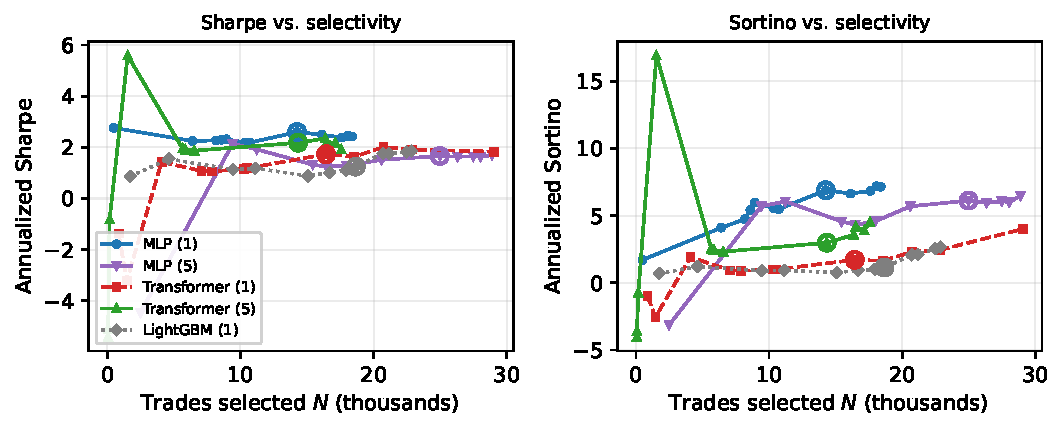
\includegraphics[width=\linewidth]{figures/selectivity_curves.pdf}
\caption{Matched-selectivity curves: annualized Sharpe (left) and Sortino (right) versus trades selected $N$ as the calibrated threshold sweeps 0.30--0.85. Open circles mark $p\ge0.5$ operating points. At matched $N$, the single-seed MLP leads throughout and the five-seed transformer leads its single-seed variant throughout.}
\label{fig:selectivity}
\end{figure}

\subsection{Multiple Testing: Deflated Sharpe Ratios}
\label{sec:dsr}
We evaluated 21 configurations on the same 2021--2026 window (the rows of Table~\ref{tab:consolidated} plus the four-denomination LightGBM, the no-history ablation, the expanding-window transformer, a 10-seed ALiBi ensemble, and the eight rejected selection-rule variants of Section~\ref{sec:calibration}); we disclose the list and use it as the trial count for the Deflated Sharpe Ratio~\cite{bailey2014deflated}, which benchmarks each observed Sharpe against the expected maximum of 21 null trials ($SR_0=2.01$ annualized) with skew and kurtosis corrections. The committed results are sobering: the five-seed transformer, the best-consistency configuration, reaches $\mathrm{DSR}=0.585$; the five-seed MLP, the P\&L leader, reaches $\mathrm{DSR}=0.250$---its Sharpe of 1.66 does not clear the multiple-testing benchmark at all. No configuration comfortably clears the conventional 0.95 bar, and the trial count is itself conservative: it excludes the five seed draws per architecture, although Table~\ref{tab:consolidated}'s single-seed MLP entry is, per Section~\ref{sec:confound}, the maximum over five seeds.
%% TODO-RERUN[67]: script 63's filename collision overwrote the MLP(1) DSR
%% artifact; when dsr_MLP_1.json lands, report it here (forward calculation
%% suggests ~0.86-0.91, still below 0.95) alongside a seed-inclusive n_trials
%% sensitivity.

\subsection{Capital-Scaled Backtest: The Deployment Lens}
\label{sec:capitalscaled}
The \$1{,}000-per-trade convention isolates selection quality but assumes unlimited capital. Under realistic sizing---\$1M starting capital, at most 1\% of available cash committed per day, equal weighting within a day, no leverage, following~\cite{glasserman2025tp2}---the picture changes decisively (Table~\ref{tab:capitalscaled}): LightGBM and the MLP remain strongly profitable while both transformer variants collapse to near-zero CAGR. The cause is payoff shape, not ranking ability: on its lowest-competition days, where per-trade capital is largest, the transformer wins \emph{more} often than LightGBM/MLP (69.9\% vs.\ 59.8\%/54.9\%) with the best discrimination (ROC-AUC 0.906 on this more balanced subset, vs.\ 0.890/0.881), but its wins are small and its losses large (payoff ratio 0.36 versus 4.09/3.54), and its best trades land on its smallest-allocation days. Flat-notional Sharpe overstates what the transformer can capture under a capital constraint---and any reversal debate conducted purely at flat notional is, from a deployment standpoint, moot: here the ordering is unambiguous.

\begin{table}[t]
\centering
\footnotesize
\begin{tabular}{lrrrr}
\toprule
Model & CAGR & Sharpe & Max DD & Calmar \\
\midrule
Unconditional & $-11.7\%$ & $-0.67$ & $-70.5\%$ & $-0.17$ \\
LightGBM & 14.6\% & 1.09 & $-6.3\%$ & 2.31 \\
MLP & 17.2\% & 1.03 & $-5.2\%$ & 3.32 \\
Transformer (plain) & 0.6\% & 0.32 & $-3.7\%$ & 0.18 \\
Transformer (ALiBi) & 0.9\% & 0.51 & $-2.5\%$ & 0.37 \\
\bottomrule
\end{tabular}
\caption{Capital-scaled backtest, 2021--2026: \$1M starting capital, 1\%-of-cash daily cap, no leverage. CAGR and drawdown do not depend on the flat-notional convention of Table~\ref{tab:consolidated}.}
\label{tab:capitalscaled}
\end{table}

\subsection{Robustness}
\label{sec:robustness}

\noindent\textbf{Strategy-level breakdown.} At matched single seed (42), K2 is the common profit source: the MLP earns \$1.21M of its \$1.41M on K2 (Sharpe 2.66 vs.\ 1.62 on T1); the single-seed transformer's entire net gain is K2 (\$717K, Sharpe 2.60) against a small T1 loss ($-$\$31K) that turns positive (\$274K) only once ensembled---another ensembling-dependent sign flip; LightGBM is the most balanced (T1 \$378K/0.85, K2 \$304K/1.74). No model's result rests on a single denomination.

\noindent\textbf{Year-by-year.} Figure~\ref{fig:annualpnl} plots test-year P\&L at matched single seed. Unconditional loses large in four of six years; the learned models stay in a narrow, mostly positive band, profitable in different years to different degrees.

\begin{figure}[t]
\centering
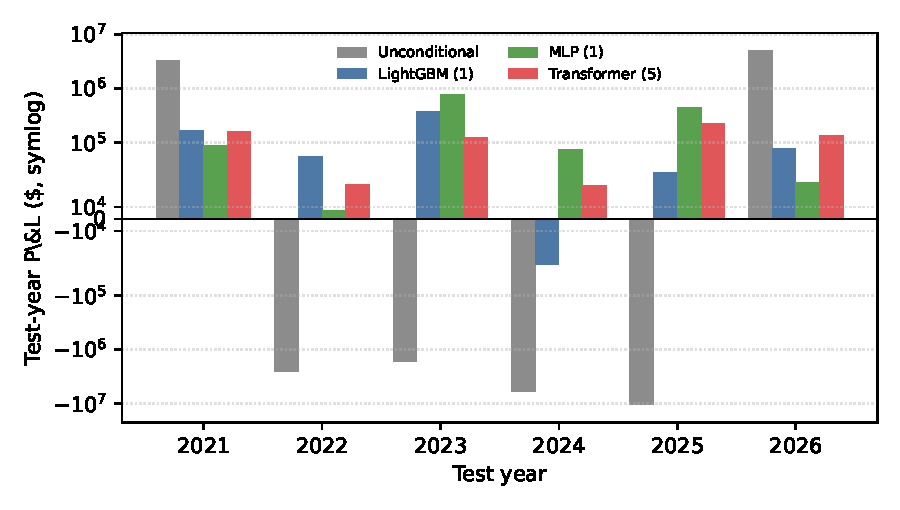
\includegraphics[width=0.66\linewidth]{figures/annual_pnl_bar_chart.pdf}
\caption{Test-year P\&L, 2021--2026, matched single seed (42), symmetric-log scale, shared axis: unconditional swings are one to two orders of magnitude larger than any learned model's.}
\label{fig:annualpnl}
\end{figure}

\noindent\textbf{Excluding the partial year.} 2026 covers $\approx$107 trading days. Re-running everything on 2021--2025 leaves every conclusion intact (MLP-1 \$1.38M/2.59; five-seed transformer \$532K/1.92; all learned models positive every year) and \emph{strengthens} the baseline contrast: unconditional worsens to $-\$17.45$M (Sharpe $-1.73$, 1/5 positive years), since 2026 was one of its two good years.

\noindent\textbf{Training window.} An expanding window earns more raw dollars for the transformer (\$734.9K vs.\ \$686.2K) from higher late-sample volume at lower quality, but loses on Sharpe in five of six years and produces the only negative-Sharpe year (2024, $-0.13$ vs.\ 1.59). We keep the three-year window.

\noindent\textbf{Execution and early assignment.} At $1.5\times$ quoted-spread slippage, all rankings and positive-year counts are unchanged; Sharpe falls 7\% (transformers) to 37\% (LightGBM). Trades whose short leg spans an ex-dividend date---early-assignment risk the expiry labels do not price---are 16--22\% of selections; LightGBM's exposed subset is net negative ($-\$33$K) while the transformer's exposed subset has a \emph{higher} win rate than its unexposed one, a divergence we report without a causal account.

\noindent\textbf{Market exposure.} Regressing each \emph{trade's} return on the underlying's return over that trade's own holding window (mean 3.6 days)---the correct test when P\&L books at exit, where a same-day daily regression has essentially no power---shows a significant \emph{positive} beta for all three models (MLP $\beta=7.2$, $t=11.5$; transformer $0.9$; LightGBM $0.7$; all $R^2<0.006$). The low $R^2$ makes the tilt noisy, not small: for the MLP, a $+1\%$ underlying move over a typical hold shifts expected trade return by $+7.2$ percentage points---roughly half its 13.7\% mean per-trade return---over a strongly rising 2021--2026 market. These strategies are long-biased, not market-neutral. Reconciling the positive realized beta with predominantly net-short entry delta (75--82\% of trades, a structural consequence of shorting the near leg) requires path-dependent effects we have not isolated, and we flag the tension openly. Separately, sensitivity to an average-IV proxy (we did not merge external VIX data) is small but significant for the transformer variants only ($r\approx0.10$, $p<0.005$). Against the \emph{unconditional} baseline, the block bootstrap finds the Sharpe improvement significant for the MLP and both transformer variants but not LightGBM (CI $[-0.03,4.13]$).

\noindent\textbf{Classification metrics.} On the pooled test population (base rate $\approx$13.8\%, identical across models by construction), Table~\ref{tab:calibration} shows no model dominating: LightGBM discriminates best (PR-AUC 0.492) despite the weakest P\&L among learned models; the plain transformer calibrates best (ECE 0.024). ROC-AUC is base-rate-invariant; we report PR-AUC because it is the more informative summary for a rare positive class, and ROC-AUC only on the balanced quiet-day subset above. The five-seed no-history ablation's PR-AUC (0.451) trails both transformer variants---seed-matched evidence that attention adds discrimination, consistent with its modest trading gain.

\begin{table}[t]
\centering
\footnotesize
\begin{tabular}{lrrr}
\toprule
Model & PR-AUC & Brier & ECE \\
\midrule
LightGBM & 0.492 & 0.086 & 0.049 \\
MLP & 0.406 & 0.096 & 0.036 \\
Transformer (plain, 5-seed) & 0.458 & 0.083 & 0.024 \\
Transformer (ALiBi, 5-seed) & 0.460 & 0.083 & 0.028 \\
No-history ablation (5-seed) & 0.451 & 0.089 & 0.046 \\
\bottomrule
\end{tabular}
\caption{PR-AUC (average precision), Brier score, and expected calibration error (10 equal-width bins) on the pooled 2021--2026 test population (base rate $\approx$13.8\%).}
\label{tab:calibration}
\end{table}

\section{Discussion and Threats to Validity}
\label{sec:limitations}

\noindent\textbf{What carries the signal.} A linear model on $F^{\ast}$ matches or beats every deep configuration except the single-seed MLP's most favorable draw; permuting the attended history costs 0.04 Sharpe; and the transformer family alone shows IV-proxy sensitivity and capital-scaled collapse. The defensible conclusion is that the episode construction and feature dictionary carry the signal, and architecture choices beyond a calibrated nonlinear (or even linear) classifier are, on this evidence, second-order---mirroring the tabular-data literature~\cite{grinsztajn2022why,shwartzziv2022tabular,gorishniy2021revisiting}.

\noindent\textbf{Validity.} The known threats, in decreasing order of concern: (i) the pooled feature-selection leakage of Section~\ref{sec:features}, affecting test years 2021--2025 through the choice (not the values) of features; (ii) the $\sim$4$\times$ base-rate shift between the early training folds and all test years, absorbed only by a one-year isotonic fit, with fold-level performance tracking the mismatch; (iii) no scale-invariant, moneyness-style price-ratio feature in $F^{\ast}$ while the underlying drifts 50--80\% across the sample; (iv) TP2 is proved for European cash-settled index options, not American SPY calls~\cite{glasserman2026tp2theory,cosma2020earlyexercise}---we treat it as an empirical hypothesis, with 16--22\% of selected trades carrying short-leg ex-dividend timing; (v) no vertical/calendar no-arbitrage pre-filter, reported elsewhere to matter little~\cite{glasserman2025tp2}. All code and derived episode/feature/label datasets will be released on acceptance; the raw vendor quote feed cannot be redistributed.

\section{Conclusion}
In a threshold-based trading pipeline, the decision rule makes the portfolio an endogenous function of the model, so model comparisons inherit an operating-point confound: five-seed ensembling moved trade counts $+75\%$ and $-13\%$ for two architectures and reversed their flat-notional Sharpe ranking, a reversal that recurs in an attention-variant ablation and shrinks a no-history ablation's apparent effect five-fold. Matched-selectivity curves, seed-dispersion intervals, honest two-sided tests with power accounting, a block bootstrap, and deflated Sharpe ratios over the disclosed 21-configuration search separate what is real here---a conditionally tradable TP2 signal recoverable by any calibrated classifier including a linear one, and a genuine within-transformer ensembling gain---from what is not: any claim that a particular architecture wins. Under capital-constrained sizing the ordering that matters for deployment is unambiguous and favors the simplest models. The open problems we leave are stated as such: per-fold feature re-selection to close the disclosed leakage, a scale-invariant feature dictionary, and reconciliation of the positive realized market beta with short entry delta.

\bibliographystyle{ACM-Reference-Format}
\begingroup
\footnotesize
\setlength{\itemsep}{0pt}
\setlength{\parskip}{0pt}
\begin{thebibliography}{27}

\bibitem{glasserman2025tp2}
Paul Glasserman, Mike Li, and Dan Pirjol. 2025. Trading TP2 Option Violations. Working paper, Columbia Business School and Stevens Institute of Technology.

\bibitem{press2022alibi}
Ofir Press, Noah A. Smith, and Mike Lewis. 2022. Train Short, Test Long: Attention with Linear Biases Enables Input Length Extrapolation. In \textit{International Conference on Learning Representations (ICLR)}.

\bibitem{glasserman2026tp2theory}
Paul Glasserman and Dan Pirjol. 2026. When Are Option Prices TP2? \textit{Mathematical Finance}. Wiley.

\bibitem{glasserman2023convexity}
Paul Glasserman and Dan Pirjol. 2023. Total Positivity and Relative Convexity of Option Prices. \textit{Frontiers of Mathematical Finance} 2, 1 (2023), 1--32.

\bibitem{ke2017lightgbm}
Guolin Ke, Qi Meng, Thomas Finley, Taifeng Wang, Wei Chen, Weidong Ma, Qiwei Ye, and Tie-Yan Liu. 2017. LightGBM: A Highly Efficient Gradient Boosting Decision Tree. In \textit{Advances in Neural Information Processing Systems (NeurIPS) 30}. 3146--3154.

\bibitem{zadrozny2002transforming}
Bianca Zadrozny and Charles Elkan. 2002. Transforming Classifier Scores into Accurate Multiclass Probability Estimates. In \textit{Proceedings of KDD}. 694--699.

\bibitem{cosma2020earlyexercise}
Antonio Cosma, Stefano Galluccio, Paola Pederzoli, and Olivier Scaillet. 2020. Early Exercise Decision in American Options with Dividends, Stochastic Volatility, and Jumps. \textit{Journal of Financial and Quantitative Analysis} 55, 1 (2020), 331--356.

\bibitem{kearns2013mlmicrostructure}
Michael Kearns and Yuriy Nevmyvaka. 2013. Machine Learning for Market Microstructure and High Frequency Trading. In \textit{High-Frequency Trading: New Realities for Traders, Markets and Regulators}. Risk Books.

\bibitem{efron1993bootstrap}
Bradley Efron and Robert J. Tibshirani. 1993. \textit{An Introduction to the Bootstrap}. Chapman \& Hall/CRC, New York.

\bibitem{kunsch1989}
Hans R. K\"unsch. 1989. The Jackknife and the Bootstrap for General Stationary Observations. \textit{Annals of Statistics} 17, 3 (1989), 1217--1241.

\bibitem{bailey2014deflated}
David H. Bailey and Marcos L\'opez de Prado. 2014. The Deflated Sharpe Ratio: Correcting for Selection Bias, Backtest Overfitting, and Non-Normality. \textit{Journal of Portfolio Management} 40, 5 (2014), 94--107.

\bibitem{harvey2016crosssection}
Campbell R. Harvey, Yan Liu, and Heqing Zhu. 2016. $\ldots$ and the Cross-Section of Expected Returns. \textit{Review of Financial Studies} 29, 1 (2016), 5--68.

\bibitem{white2000reality}
Halbert White. 2000. A Reality Check for Data Snooping. \textit{Econometrica} 68, 5 (2000), 1097--1126.

\bibitem{hansen2005spa}
Peter R. Hansen. 2005. A Test for Superior Predictive Ability. \textit{Journal of Business \& Economic Statistics} 23, 4 (2005), 365--380.

\bibitem{bouthillier2021accounting}
Xavier Bouthillier et al. 2021. Accounting for Variance in Machine Learning Benchmarks. In \textit{Proceedings of Machine Learning and Systems (MLSys)} 3.

\bibitem{dodge2019show}
Jesse Dodge, Suchin Gururangan, Dallas Card, Roy Schwartz, and Noah A. Smith. 2019. Show Your Work: Improved Reporting of Experimental Results. In \textit{Proceedings of EMNLP-IJCNLP}. 2185--2194.

\bibitem{melis2018state}
G\'abor Melis, Chris Dyer, and Phil Blunsom. 2018. On the State of the Art of Evaluation in Neural Language Models. In \textit{International Conference on Learning Representations (ICLR)}.

\bibitem{lucic2018gans}
Mario Lucic, Karol Kurach, Marcin Michalski, Sylvain Gelly, and Olivier Bousquet. 2018. Are GANs Created Equal? A Large-Scale Study. In \textit{Advances in Neural Information Processing Systems (NeurIPS) 31}. 698--707.

\bibitem{agarwal2021deep}
Rishabh Agarwal, Max Schwarzer, Pablo Samuel Castro, Aaron Courville, and Marc G. Bellemare. 2021. Deep Reinforcement Learning at the Edge of the Statistical Precipice. In \textit{Advances in Neural Information Processing Systems (NeurIPS) 34}. 29304--29320.

\bibitem{grinsztajn2022why}
L\'eo Grinsztajn, Edouard Oyallon, and Ga\"el Varoquaux. 2022. Why Do Tree-Based Models Still Outperform Deep Learning on Typical Tabular Data? In \textit{Advances in Neural Information Processing Systems (NeurIPS) 35 Datasets and Benchmarks}.

\bibitem{shwartzziv2022tabular}
Ravid Shwartz-Ziv and Amitai Armon. 2022. Tabular Data: Deep Learning Is Not All You Need. \textit{Information Fusion} 81 (2022), 84--90.

\bibitem{gorishniy2021revisiting}
Yury Gorishniy, Ivan Rubachev, Valentin Khrulkov, and Artem Babenko. 2021. Revisiting Deep Learning Models for Tabular Data. In \textit{Advances in Neural Information Processing Systems (NeurIPS) 34}. 18932--18943.

\bibitem{shaw2018self}
Peter Shaw, Jakob Uszkoreit, and Ashish Vaswani. 2018. Self-Attention with Relative Position Representations. In \textit{Proceedings of NAACL-HLT}. 464--468.

\bibitem{raffel2020t5}
Colin Raffel et al. 2020. Exploring the Limits of Transfer Learning with a Unified Text-to-Text Transformer. \textit{Journal of Machine Learning Research} 21, 140 (2020), 1--67.

\bibitem{ying2021graphormer}
Chengxuan Ying et al. 2021. Do Transformers Really Perform Badly for Graph Representation? In \textit{Advances in Neural Information Processing Systems (NeurIPS) 34}. 28877--28888.

\bibitem{li2024fire}
Shanda Li et al. 2024. Functional Interpolation for Relative Positions Improves Long Context Transformers. In \textit{International Conference on Learning Representations (ICLR)}.

\bibitem{bali2023option}
Turan G. Bali, Heiner Beckmeyer, Mathis M\"orke, and Florian Weigert. 2023. Option Return Predictability with Machine Learning and Big Data. \textit{Review of Financial Studies} 36, 9 (2023), 3548--3602.

\end{thebibliography}
\endgroup

\end{document}
